\documentclass[a4paper, 12pt]{article}

\usepackage[slovak]{babel}
\usepackage[text={17cm, 24cm}, top=3cm, left = 2cm]{geometry}
\usepackage[T1]{fontenc}
\usepackage[utf8]{inputenc}
\usepackage{times}
\usepackage{graphics}
\usepackage{wrapfig}

\begin{document}
	\begin{titlepage}
		
		\begin{center}
			\textsc{{\LARGE Vysoké učení technické v Brně \\[0.5em]}  {\LARGE Fakulta informačních technologií}} \\
			\vspace{\stretch{0.382}}
			{\Large Formálne jazyky a prekladače  -- Projekt \\[0.6em]}
			{\huge Prekladač pre jazyk ZIG} \\[0.6em]
			{\large Tým xluptas00 varianta TRP-izp}
			\vspace{\stretch{0.618}}
			
		\end{center}
		\begin{flushright}
			{ \textbf{Bodové rozdelenie:} 25/25/25/25\% \hfill \textbf{Vedúci: }Samuel Lupták (xluptas00)} \\
			{ \textbf{Implementované rozšírenia:} žiadne\hfill  Petr Nemec (xlogin00)} \\
			{ \hfill  Lukáš (xlogin00)} \\
			{\today \hfill Mário Klopan (xlogin00)}
		\end{flushright}
		
	\end{titlepage}
	
	\section{Návrh}
	\noindent Prekladač sa skladá z 3~hlavných častí a 4~pomocných dátových štruktúr.\\
	\textbf{Hlavné časti} prekladaču (a ich podčasti):
	\begin{itemize}
		\item Lexikálny analyzátor \footnote[1]{Ďalej len \textit{skener}}
		\item Dvojprechodový syntaktický a sématický analyzátor \footnote[2]{Ďalej len \textit{parser}}
		\begin{itemize} 
			\item Analýza kódu pomocou rekurzívneho zostupu
			\item Analýza výrazov pomocou precedenčnej analýzi 
		\end{itemize}
		\item Generátor výsledného kódu
	\end{itemize}
	
	\noindent\textbf{Pomocné štruktúry} použité v prekladači:
		\begin{itemize}
		\item  Tabulka s rozptýlenými položkami s implicitným zreťazením položiek \footnote[3]{Ďalej len \textit{hašovacia tabulka}}
		\item Abstraktný syntaktický strom \footnote[4]{Ďalej len \textit{ASS}}
		\item Zásobník
		\item Fronta
	\end{itemize}
	
	\noindent \textbf{Využitie} jednotlivých štruktúr je nasledovné:\\
	\par\textit{Hašovacia tabulka: } Bola použítá pre implementáciu tabulky symbolov. Podmienka pre implicitné zreťazenie nám 
	robila mierny problém, pretože teoreticky nekonečný počet identifikátorov sa nemestí do konečne velkej tabulky \\
	\par\textit{ASS: } Slúži na komunikáciu medzi parserom a generátorom kódu\\
	\par\textit{Zásobník: } Je využitý precedenčnou analýzou, ktorá ho používa na spracovanie výrazov\\
	\par\textit{Fronta: } Má význam pri dvojprechodovej analýze ako uložisko tokenov. Pre dvojprechodovú analýzu sme sa rozhodli po
	zistení, že definicia funkcie nemusí lexikálne predchádzať jej volaniu.
	
	\newpage
	\section{Popis komunikácie}
	\subsection{Diagram}
	
	\begin{figure}[ht]
		\begin{center}
			\scalebox{0.5}{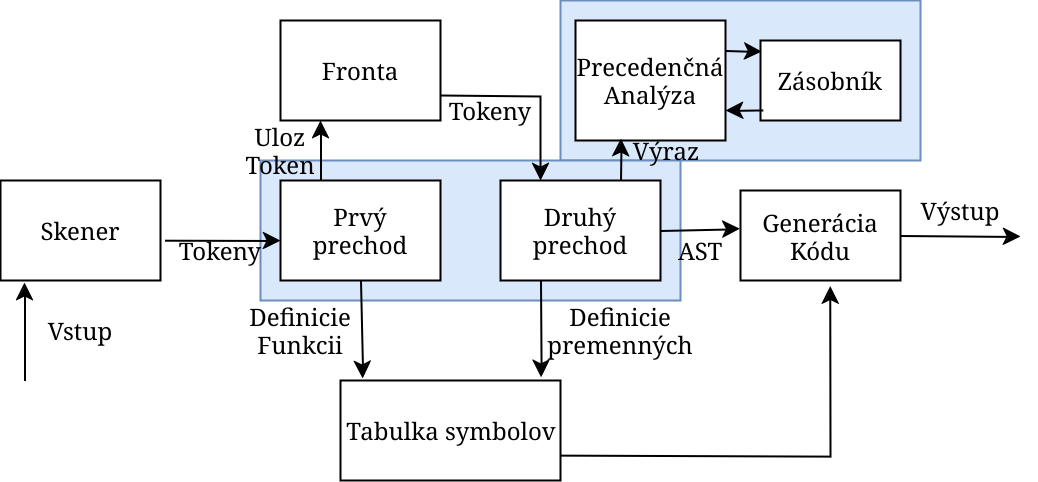
\includegraphics{Untitled Diagram.png}}
		\end{center}
	\end{figure}
	\subsection{Stručný popis}
	Bolo by vhodné začať tým, že parser (modrá časť diagramu) inicializuje všetky operácie v prekladači.  
	Preklad začína vložením programu v jazyku zig na
	 vstup. Skener (Na zavolanie) postupne fragmentuje vstup na jednotlivé lexémi a posiela ich vo forme tokenov do parseru.  Ako bolo už spomenuté, tak parser je dvojprechodový. Tokeny idú najprv cez prvý prechod, ktorý kontroluje syntax a sematiku iba pre hlavičky funkcií, ktoré následne ukladá do tabulky symbolov, aby informácie o nich boli dostupné v druhom prechode. Prvý prechod ukladá všetky prečítané tokeny do fronty. Z fronty si tokeny po jednom berie druhý prechod, ktorý kontroluje syntax a sématiku pre ostatok kódu. V prípade že v kóde sa nachádza výraz, zavolá sa precedenčná analýza ktorá tento výraz s pomocov zásobníku spracuje. Druhý prechod zároveň pridáva definované premenné do tabulky symbolov  (Samotnú tabulku symbolov však aj využíva, napr. pre kontrolu redefinície).  Počas druhého prechodu sa zároveň vytvára ASS ktorý po úspešnom dokončení analýzi slúži ako výstup a zároveň vstup do generátoru kódu. Generátor kódu s pomocou tabulky symbolou generuje cieľový kód.
	 	
	\newpage
	\section{Implementácia}
	\textbf{Skener: }\textit{lexer.*, token.h}(xlogins)\\ 
	\textbf{Parser: }\textit{syntax.*, queue\_fill.*, precedence.*} (xluptas00, xlogins)\\
	\textbf{Generátor kódu: }\textit{code\_gen.*}(xlogins)\\
	\textbf{Hašovacia tabulka: }\textit{symtable.*}(xluptas00)\\
	\textbf{ASS: }\textit{tree.*}(xlogins)\\
	\textbf{Zásobník: }\textit{stack.*}(xlogins)\\
	\textbf{Fronta: }\textit{queue.*} (xluptas00)\\
	\textbf{Ostatné časti: }\textit{error.*} (xluptas00)\\
	\par Implementácia dátových štruktúr sa nachádza v jednotlitvých súboroch pomenovaných podla danej štruktúry.
	\par Implementácia častí samotného prekladača spočíva v súboroch skeneru, parseru, generátoru a súboru error.*, ktorý 
	implementuje základné pracovanie s chybami. Prvý prechod je implementovaný v súboroch queue\_fill.* a druhý prechod je
	implementovaný v súboroch syntax.*. syntax.c zároveň obsahuje funkciu Main. Prílohy A, B, C, D ukazujú využitú teóriu, ktorá slúžila ako podklad pre jednotlivé časti prekladaču.
	
	\subsection{Strom}
	\begin{wrapfigure}{l}{0.4\textwidth}
		\scalebox{0.25}{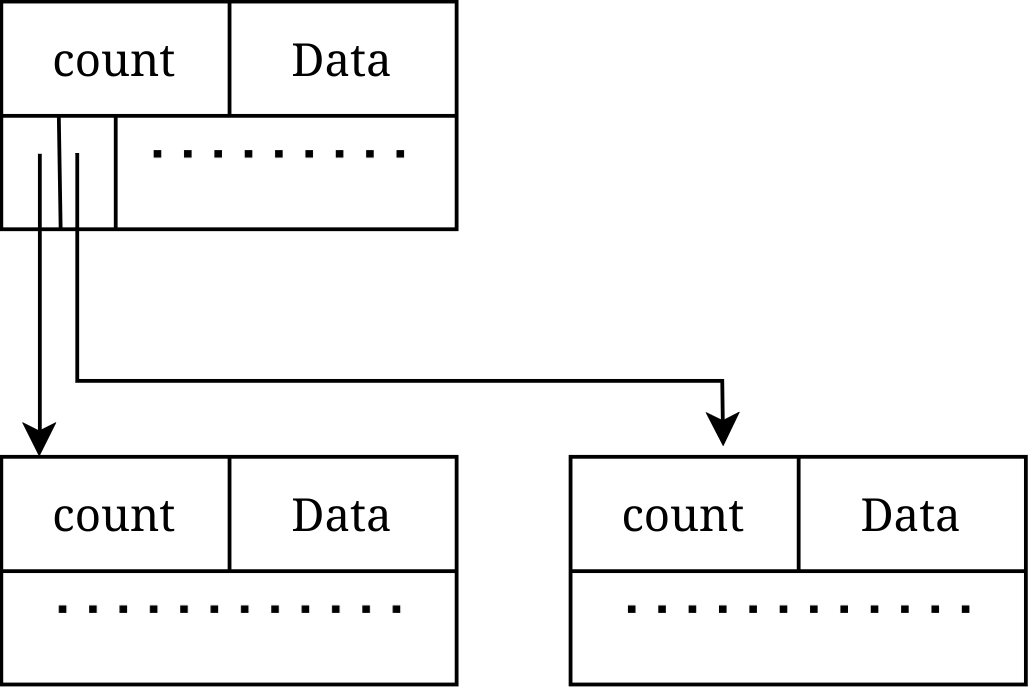
\includegraphics{Untitled Diagram(1).png}}
	\end{wrapfigure}
	Pre kompletnosť sme sa rozhodli vizualizovať ASS, ktorý sme navrhli pre tento prekladač.
	Ako je vidno na diagrame, tak každý uzol obsahuje 3 hlavné časti a to sú: \textit{count, data, children}. Kde \textit{count}
	určuje počet detí ktoré daný uzol má. Hlavná časť, \textit{data}, v sebe uchováva data potrebné na správne generovanie kódu
	(viac viď. tree.*). Posledná časť \textit{children} je pole ukazovaťelov na deti. Pre konkrétne prípady ako sa strom využíva viď.
	syntax.c alebo precedence.c\\
	
	\subsection{Neštandardné riešenia}
	\textbf{Veľkosť tabulky symbolov: } Jediná implementačná anomália v rámci dátových štruktúr je 
	statické obmedzenie veľkosti tabulky symbolov na 
	1000 položiek z dôvodu požadovanej implementácie pomocou implicitného zreťazenia položiek. Veľkosť 1000 bola zvolená 
	na základe informácií, že viac ako 1000 položiek sa v žiadom teste nebude nachádzať. Uvedomujeme si že omnoho lepšie riešenie by bola tabulka symbolov s explicitným zreťazením položiek.\\
	\textbf{Úroveň zanorenia v tabulke symbolov: }
	\newpage
	
	\section{Práca v tíme}
	
	\newpage
	\section{PRÍLOHA A - Konečný automat}
	
	\newpage
	\section{PRÍLOHA B - LL1 gramatika}
	
	\newpage
	\section{PRÍLOHA C - LL1 tabulka}
	
	\newpage
	\section{PRÍLOHA D - Precedenčná tabulka}
	
\end{document}